
%(BEGIN_QUESTION)
% Copyright 2007, Tony R. Kuphaldt, released under the Creative Commons Attribution License (v 1.0)
% This means you may do almost anything with this work of mine, so long as you give me proper credit

Suppose we wished to build a liquid flow control loop using FOUNDATION Fieldbus H1 devices.  Of course, we will need a flow transmitter to measure liquid flow, and a flow control valve to throttle the liquid, but we will not need a separate controller device because all Fieldbus transmitters and valve positioners have the capacity to implement control algorithms themselves.  The physical layout of our flow control system might look like this:

$$\includegraphics[width=15.5cm]{i02442x01.eps}$$

The control algorithm, consisting of function blocks interconnected to perform all the necessary data conversion and processing tasks, will look like this:

$$\includegraphics[width=15.5cm]{i02442x02.eps}$$

Does it matter whether the PID function block resides within the Fieldbus transmitter or within the Fieldbus valve positioner?  Either configuration is possible, but are they equally practical?  Why or why not?  Both options are shown in the following illustrations:

$$\includegraphics[width=15.5cm]{i02442x03.eps}$$

\vskip 20pt

$$\includegraphics[width=15.5cm]{i02442x04.eps}$$

\underbar{file i02442}
%(END_QUESTION)





%(BEGIN_ANSWER)

With the PID block resident in the transmitter, both the PID output and the back calculation signal must be communicated over the Fieldbus network.  With the PID block resident in the valve positioner, only the PV signal needs to be communicated over the Fieldbus network.  Thus, it is customary to place the PID function block in the final control element rather than in the transmitter to minimize scheduled (cyclic) Fieldbus communications.  This allows for faster macrocycle times.

\vskip 10pt

You should never place the PID block in the host (DCS) system unless that host is an actual Fieldbus device whose processing time is included in the LAS schedule.  In most systems, this is not the case.  If PID calculations are being done in a non-Fieldbus device, those calculations will not necessarily be available to the other Fieldbus devices when needed, causing non-deterministic behavior.

\vskip 10pt

On a similar note, while it is possible to place the PID block for a control loop inside a field device for a completely different loop (e.g. the PID control block for flow control loop 101 residing within temperature transmitter 106, on the same segment), this may cause problems later on when that other field device fails or must be removed for maintenance.  The totally distributed nature of FOUNDATION Fieldbus processing makes loop documentation very challenging, because it is now possible for ``unrelated'' field devices to be given critical roles in control loops!

%(END_ANSWER)





%(BEGIN_NOTES)


%INDEX% Fieldbus, FOUNDATION (H1): grouping function blocks by device

%(END_NOTES)


